\section{An \texorpdfstring{\boldmath$\Omega(n^{3/2 - \epsilon})$}{Omega(n\^(3/2-epsilon))} Conditional Lower Bound for Average Linkage HAC}\label{sec:worklb}

In this section, we show an $\Omega(n^{3/2 - \epsilon})$ conditional lower bound on the time required to solve average linkage HAC on general weighted graphs. Specifically, we show this lower bound assuming the Combinatorial Boolean Matrix Multiplication (BMM) conjecture, a central conjecture in fine-grained complexity about the time required to multiply two $n \times n$ boolean matrices~\cite{williams2010subcubic, abboud2024faster}.
%\enote{We should define boolean matrix multiplication; we use it later in the corollary}

\begin{conjecture}[Combinatorial BMM]\label{conj:bmm}
Combinatorial algorithms cannot solve Boolean Matrix Multiplication in time $O(n^{3-\epsilon})$ for $\epsilon > 0$.
\end{conjecture}
\noindent We refer to~\cite{abboud2024faster} for an in-depth discussion of the somewhat informal notion of ``combinatorial'' algorithms and more on Conjecture~\ref{conj:bmm} and its history.

In this work we will make use of an equivalent characterization of the BMM conjecture due to \cite{williams2010subcubic}. Specifically, \cite{williams2010subcubic} shows that the BMM problem is sub-cubically equivalent to the Triangle Detection problem: the problem of deciding whether or not an input graph $G$ contains a triangle (i.e., cycle of $3$ vertices). The following summarizes this result.
\begin{theorem}[Theorem 1.3 of \cite{williams2010subcubic}]\label{thm:bmmeq}
    Combinatorial algorithms cannot solve Triangle Detection in time $O(n^{3-\epsilon})$ for  $\epsilon > 0$ unless \Cref{conj:bmm} is false.
\end{theorem}
Thus, we give a reduction from Triangle Detection to average linkage HAC. Our reduction will quadratically increase the number of vertices of the input Triangle Detection instance, and therefore give an $\Omega(n^{3/2 - \epsilon})$ lower bound for average linkage HAC. In the rest of this section, we show the following quadratic-blowup reduction from Triangle Detection to average linkage HAC.
%

\begin{theorem}\label{thm:lbreduction}
Given a Triangle Detection instance on graph $G$ with $t$ vertices and $m$ edges, there is a reduction that runs in $O(t^2)$ time and constructs an instance of average linkage HAC on graph $G'$ with $t + t^2$ vertices and $t^2 + m$ edges. 
Furthermore, given the sequence of merges performed by average linkage HAC on $G'$, we can solve Triangle Detection on $G$ in time $O(t^2)$.
\end{theorem}

As a corollary of this reduction and \Cref{thm:bmmeq}, we obtain the following conditional lower-bound on the running time of HAC.
%ruling out near-linear work algorithms for average linkage HAC on sparse graphs conditional on Conjecture~\ref{conj:bmm}.

\mainLowerSeq*

As a second corollary, we obtain a conditional lower-bound in terms of the optimal running time of matrix multiplication for two $n \times n$ binary matrices. 
Matrix multiplication can be solved in time $O(n^{\omega})$ where $2 \leq \omega < 2.3716$~\cite{williams2024new}. 
An extensive line of research on matrix multiplication over the past thirty years has only improved $\omega$ from $2.376$ to $2.3716$, with the current state-of-the-art being due to a very recent result of Williams et al.~\cite{williams2024new} (for a subset of the historical advances in this area see, e.g., \cite{coppersmith1982asymptotic, le2012faster, alman2021refined, williams2012multiplying}).
The fastest known algorithm for triangle detection works by simply reducing the problem to matrix multiplication and therefore runs in $O(n^{\omega})$ time.
Surprisingly, despite triangle detection only returning a single bit (whether a triangle exists or not in $G$), the problem can be used to give a sub-cubic reduction for boolean matrix multiplication (where the output is $n^2$ bits).
In particular, an algorithm for triangle detection running in time $O(n^{3-\delta})$ for some $\delta > 0$ yields an algorithm for matrix multiplication in time $O(n^{3-\delta/3})$~\cite{williams2010subcubic}.
Using this fact, we can derive a conditional lower bound based on the value of $\omega$.

\workmatmul*



%\lnote{Not very happy with the below formulation.}
%\hnote{How about we state a theorem about the  actual reduction and the quadratic blow-up, and then two corollaries about its implications? Also, in the corollary below, I would mention matrix multiplication rather than triangle detection. I would then add a couple of sentences for the non-familiar reader that, while we do not know if $\omega$ has to be greater than two, thirty years of extensive research has only improved it from 2.376 to 2.372.}
%Another consequence of our reduction is that a non-combinatorial algorithm for average linkage HAC running in $O(n^{\omega/2 - \epsilon})$ time for any $\epsilon > 0$ would imply an algorithm for triangle detection in $O(n^{\omega - \epsilon'})$ time for some $\epsilon' > 0$.

An interesting open question is whether there are faster non-combinatorial algorithms that can leverage fast matrix multiplication or Strassen-like techniques and improve over the $\Omega(n^{3/2 - \epsilon})$ barrier for combinatorial algorithms for average linkage HAC.

\subsection{Reduction}
We now prove Theorem~\ref{thm:lbreduction} by
giving a quadratic-time reduction from triangle detection to average linkage HAC.
The reduction is loosely inspired by a recent lower-bound result for multidimensional range queries~\cite{lau2021algorithms}.
%\knote{Mention that the LB is loosely based on the range-minimum paper}
The input to the reduction is an unweighted graph $G$ on $t$ vertices with $m$ edges; the problem is to detect whether $G$ has a triangle.
To do this, we will construct a HAC instance on an edge-weighted graph $G'$ with $t + t^2$ vertices and $t^2 + m$ edges. 
%\hnote{There are $t^2+t$ vertices, right?}
We will show that the specific way in which an exact HAC algorithm merges the edges in this instance reveals whether or not $G$ has a triangle.

\paragraph{Constructing $G'$}
Let $N_{G}(v)$ denote the neighbors of a vertex $v \in G$ (note that $v \notin N_{G}(v)$).
%\knote{incl/excl $v$?}
We define $G'$ as follows. 
We start by adding all vertices and edges from $G$, that is the $t$ vertices $v_1, \ldots, v_t$ from $G$, including all of their incident edges $N_{G}(v_i)$.
We call these the {\em core} vertices. 
The initail weight of the edges between any two core vertices is set to $1$.

In addition to the core vertices, we add an additional $t^2$ {\em leaf} vertices that we connect to the core vertices with specific edge weights.
We add the $t^2$ leaf vertices over a sequence of $t$ {\em rounds} where the $i$-th round connects one new leaf vertex to every core vertex.
The weights to the newly added leaves depend on the neighbors of the node $v_i$ in the original graph $G$, and are set as follows:
\begin{enumerate}[label=(\textbf{\arabic*})]
\item A core vertex $v_j$ is connected to its new leaf with an edge of weight $(1/i) - \epsilon$ if $v_j \in N_{G}(v_i)$.\label{typeone}
\item A core vertex $v_j$ is connected to its new leaf with an edge of weight $(1/i) + \epsilon$ if $v_j \notin N_{G}(v_i)$.\label{typetwo}
\end{enumerate}

\noindent See \Cref{fig:HACSeqRed} for an illustration of our reduction.
\begin{figure}[h]
    \centering
    \begin{subfigure}[b]{0.25\textwidth}
        \centering
        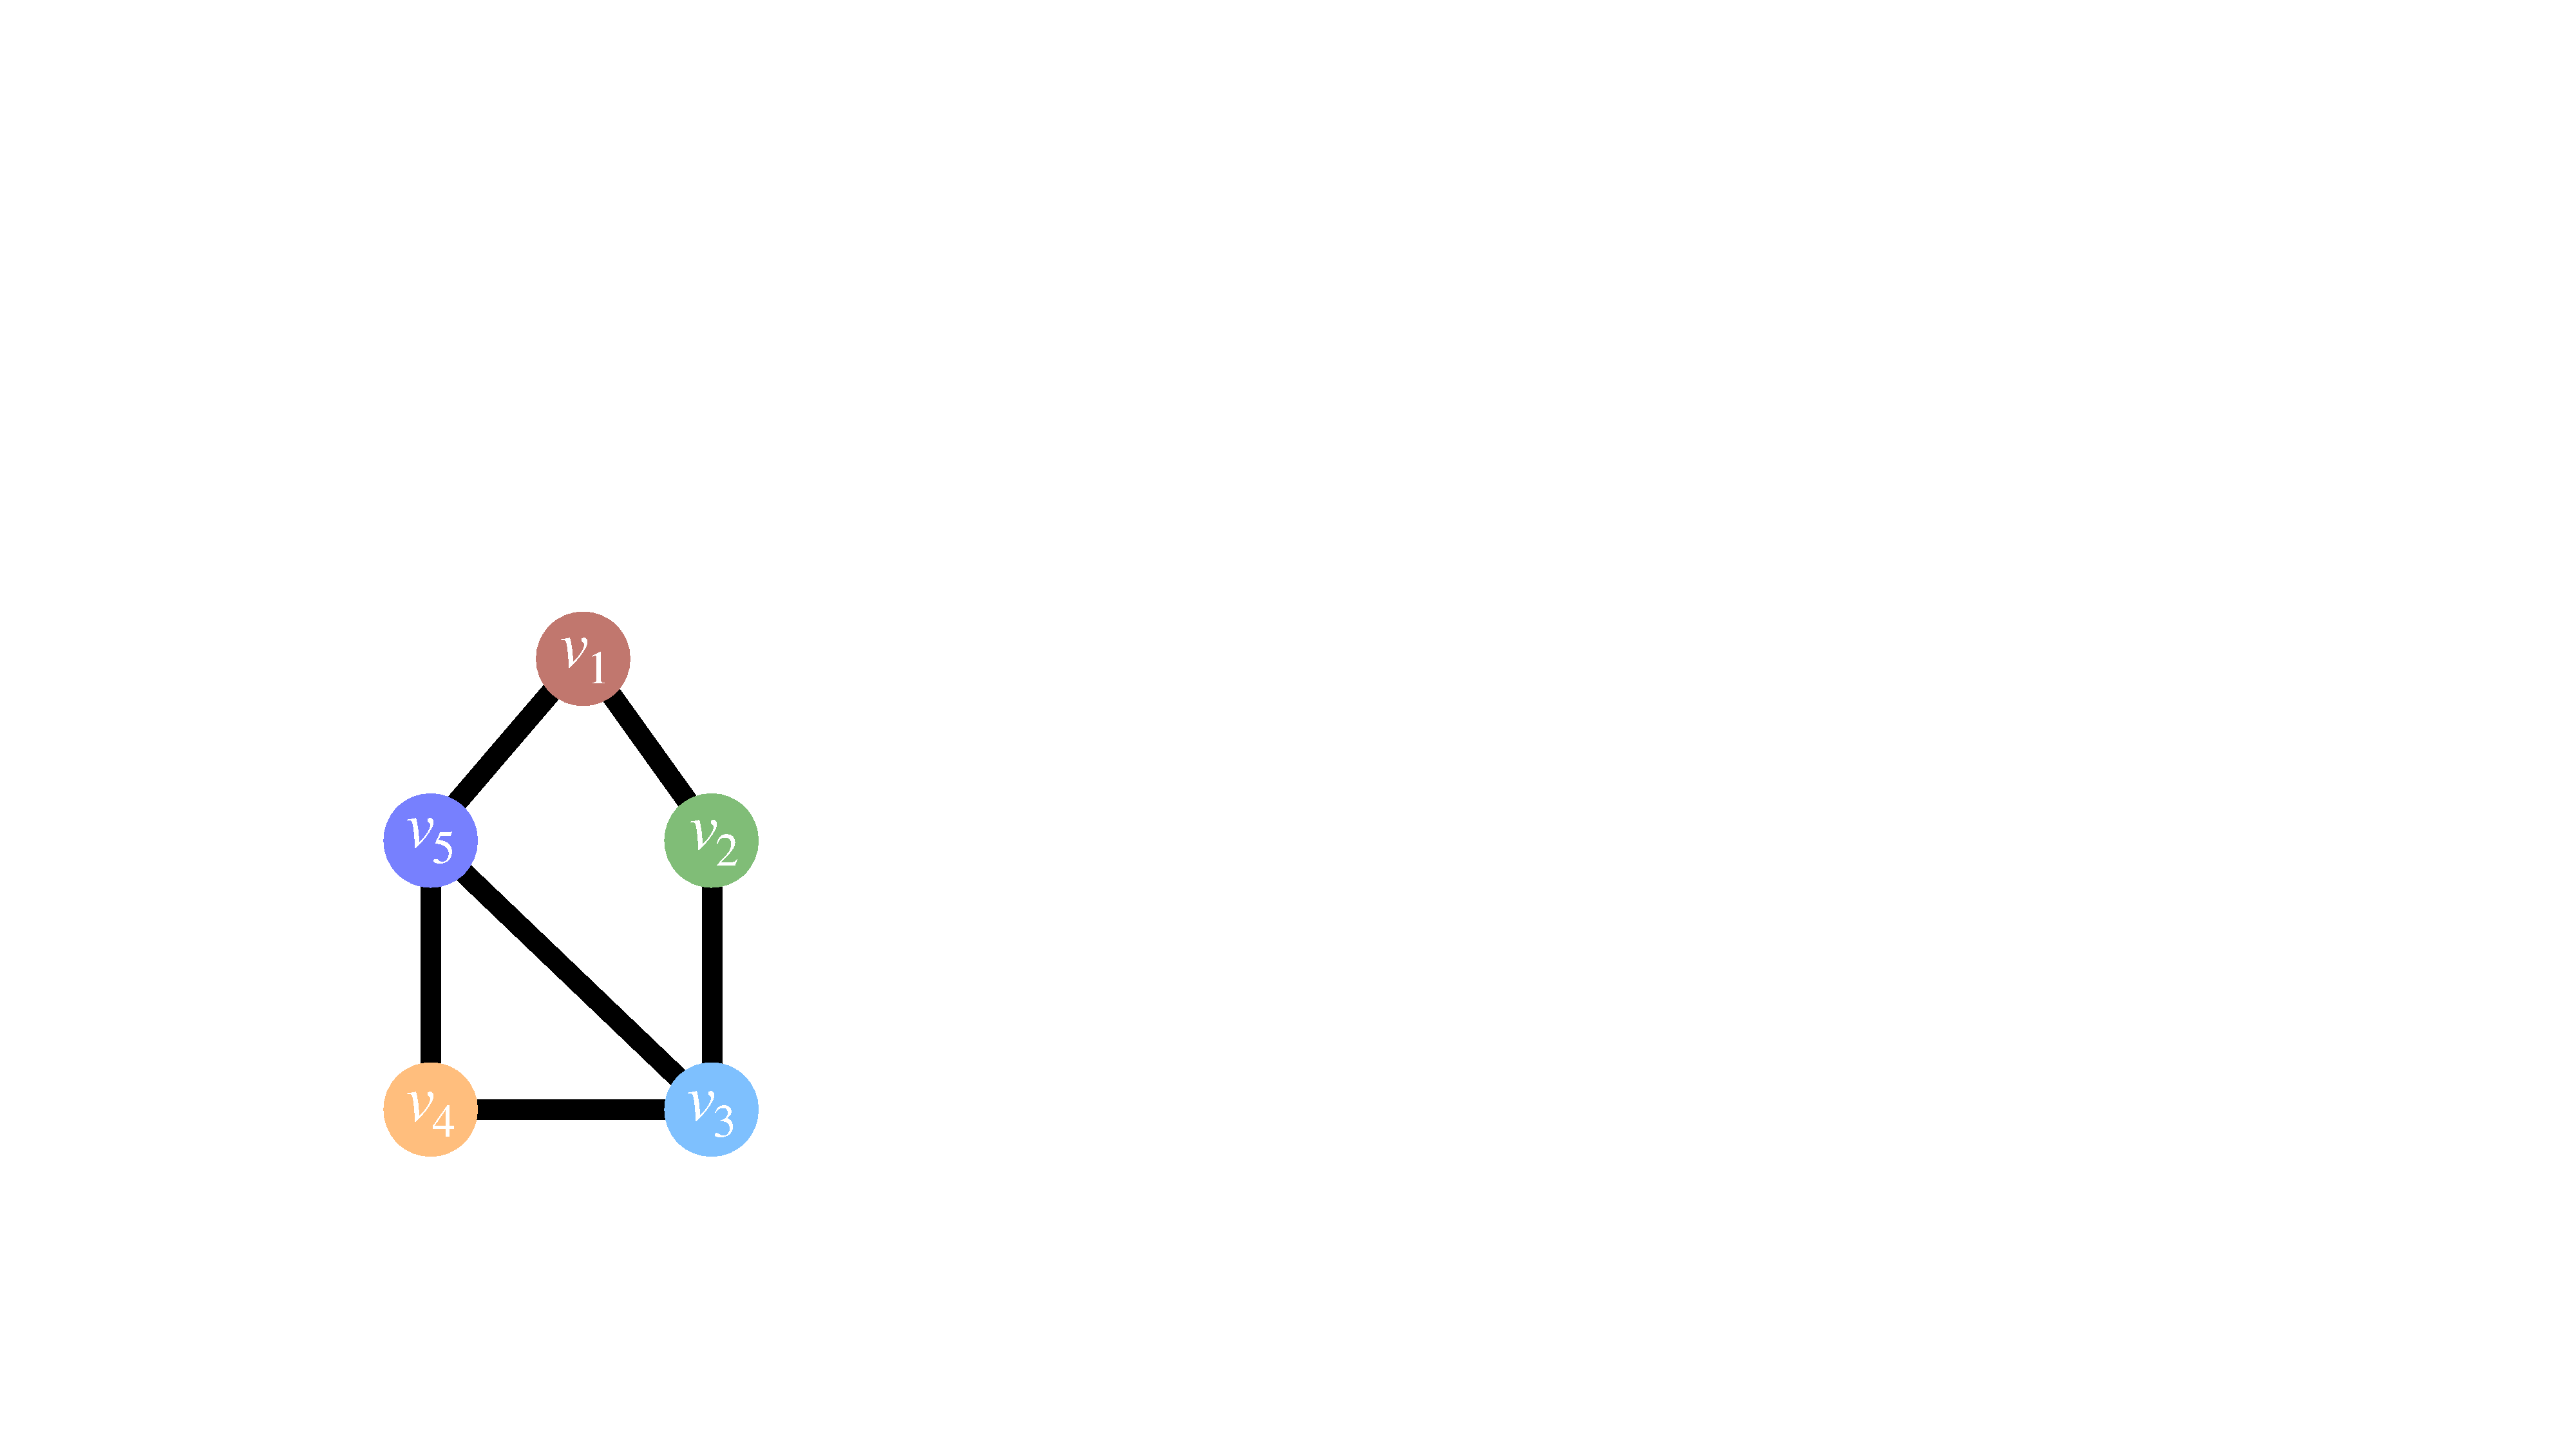
\includegraphics[width=\textwidth,trim=0mm 0mm 370mm 160mm, clip]{./figures/CBMMRed1.pdf}
        \caption{Input $G$.}\label{sfig:CBMMRed1}
    \end{subfigure} \hfill
       \begin{subfigure}[b]{0.25\textwidth}
        \centering
        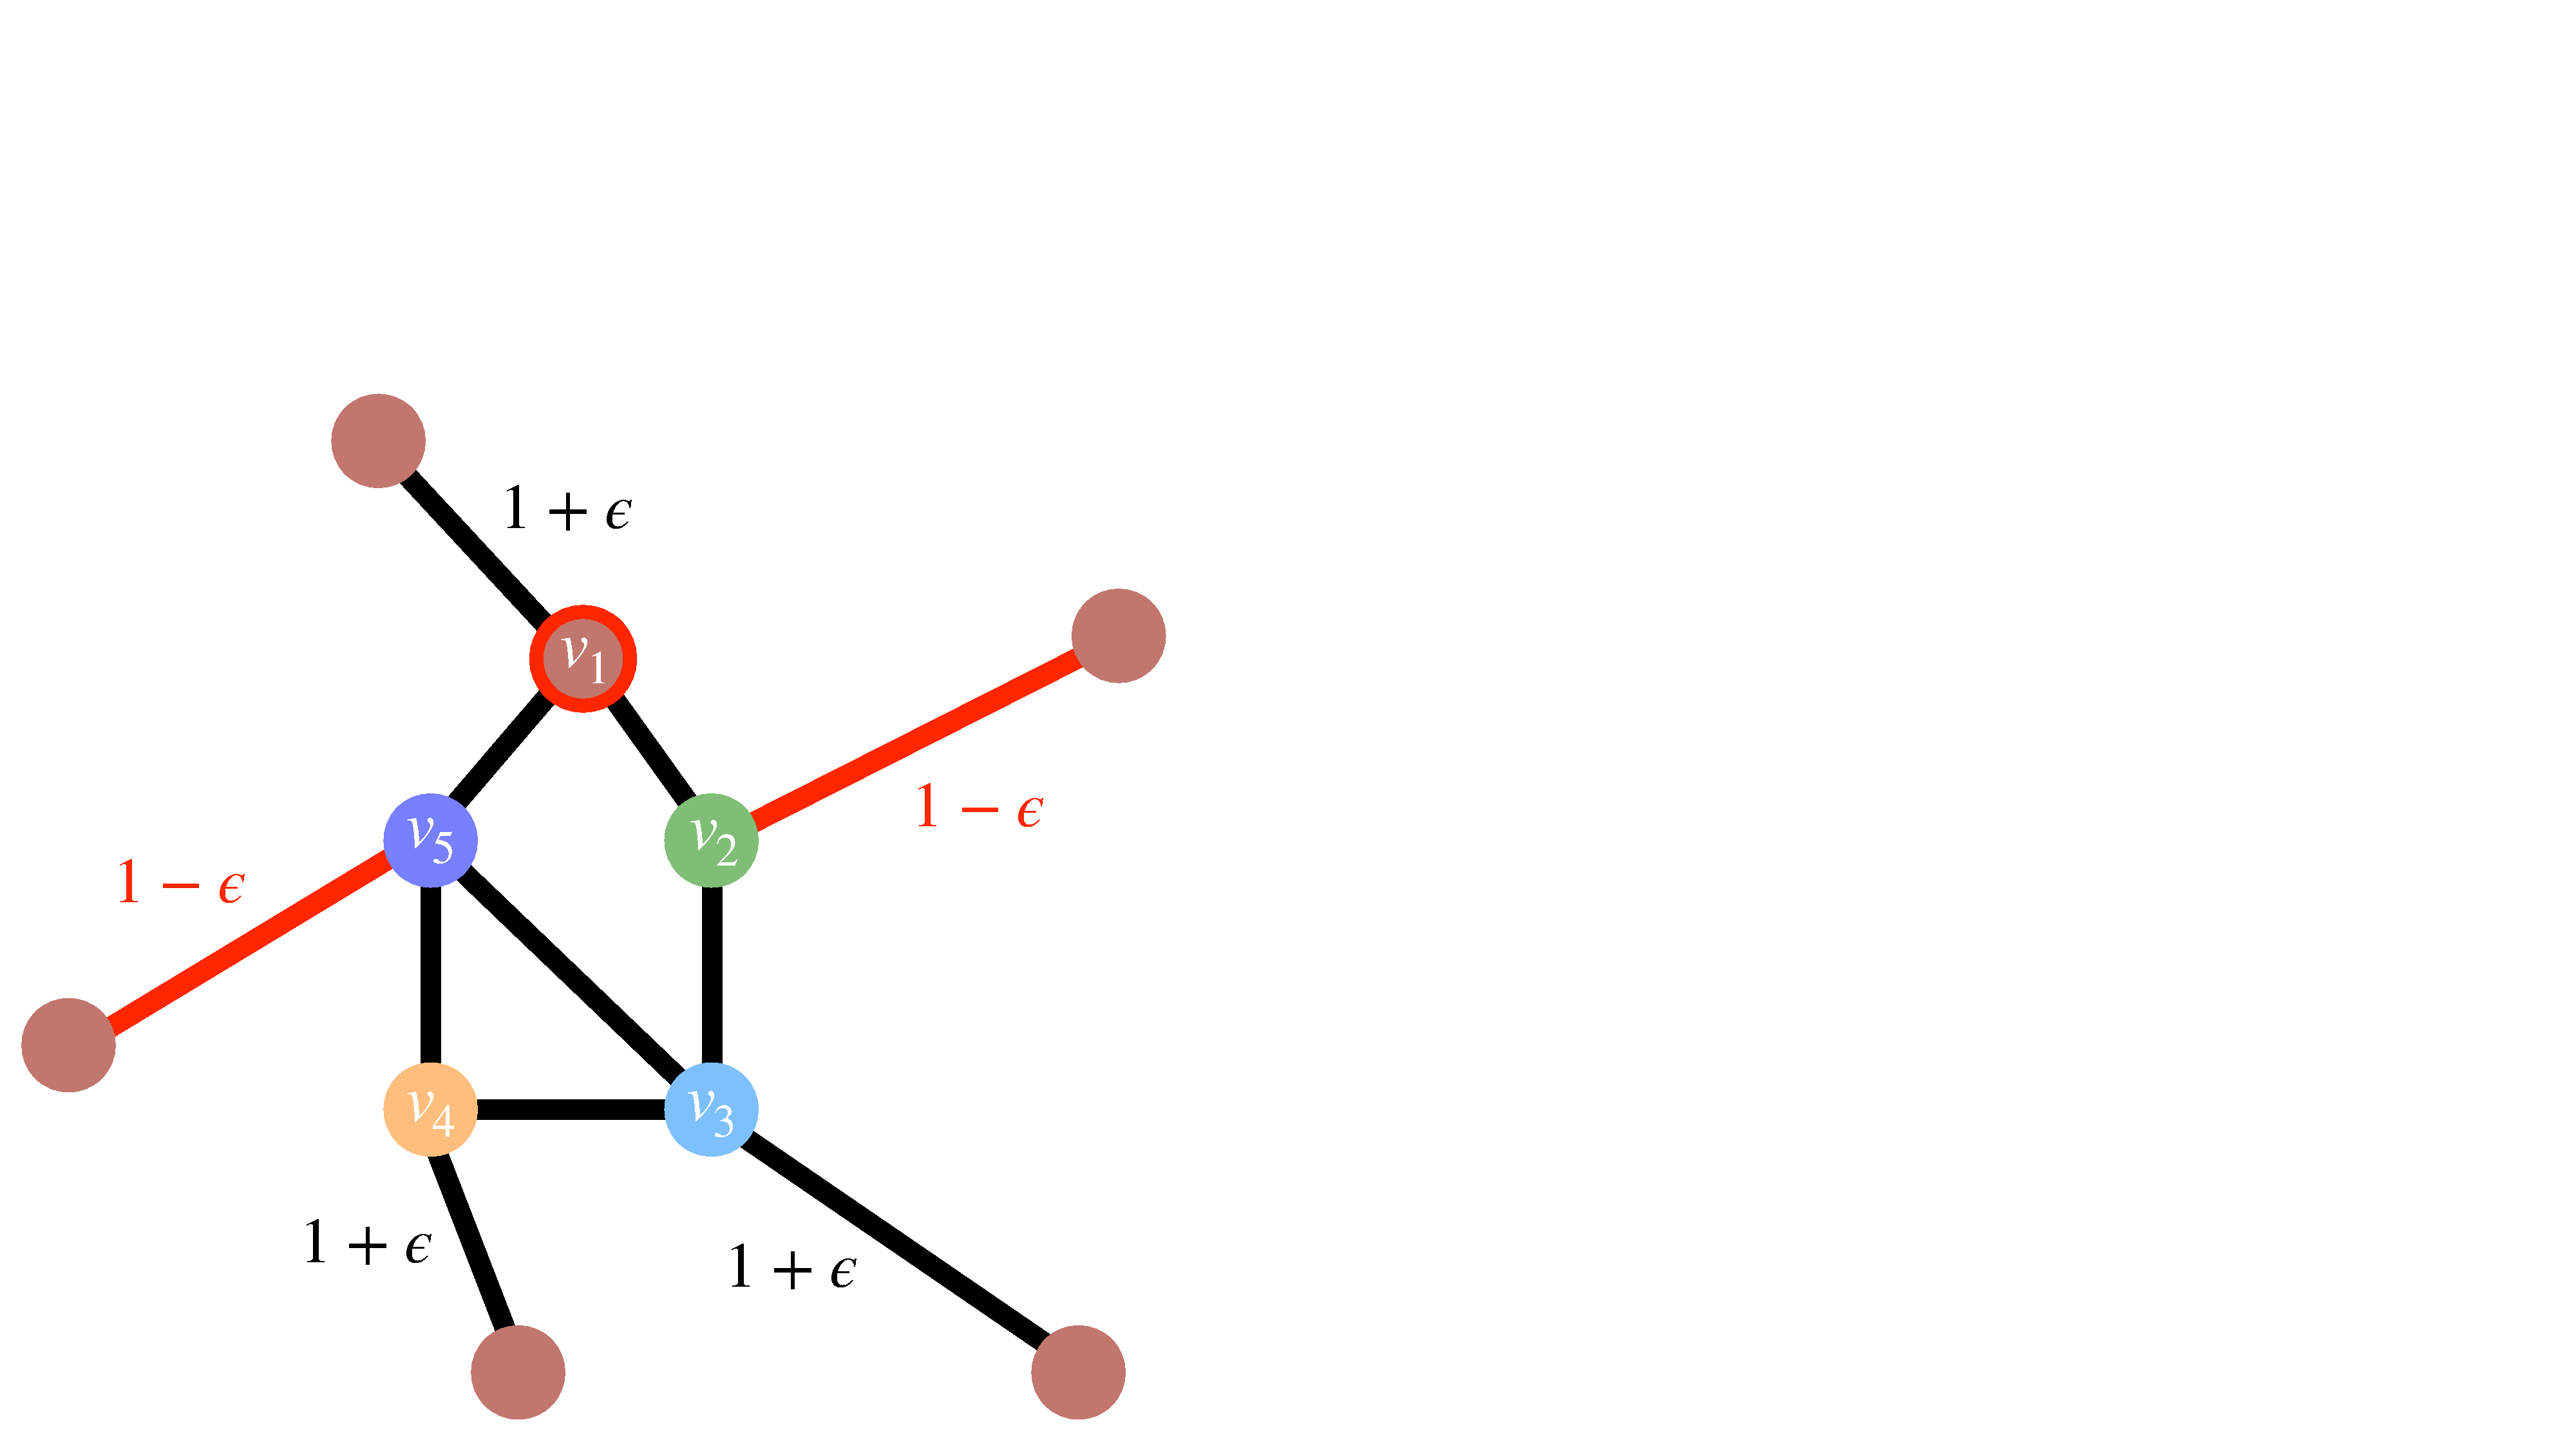
\includegraphics[width=\textwidth,trim=0mm 0mm 370mm 80mm, clip]{./figures/CBMMRed2.pdf}
        \caption{Round $1$.}\label{sfig:CBMMRed2}
    \end{subfigure} \hfill
       \begin{subfigure}[b]{0.25\textwidth}
        \centering
        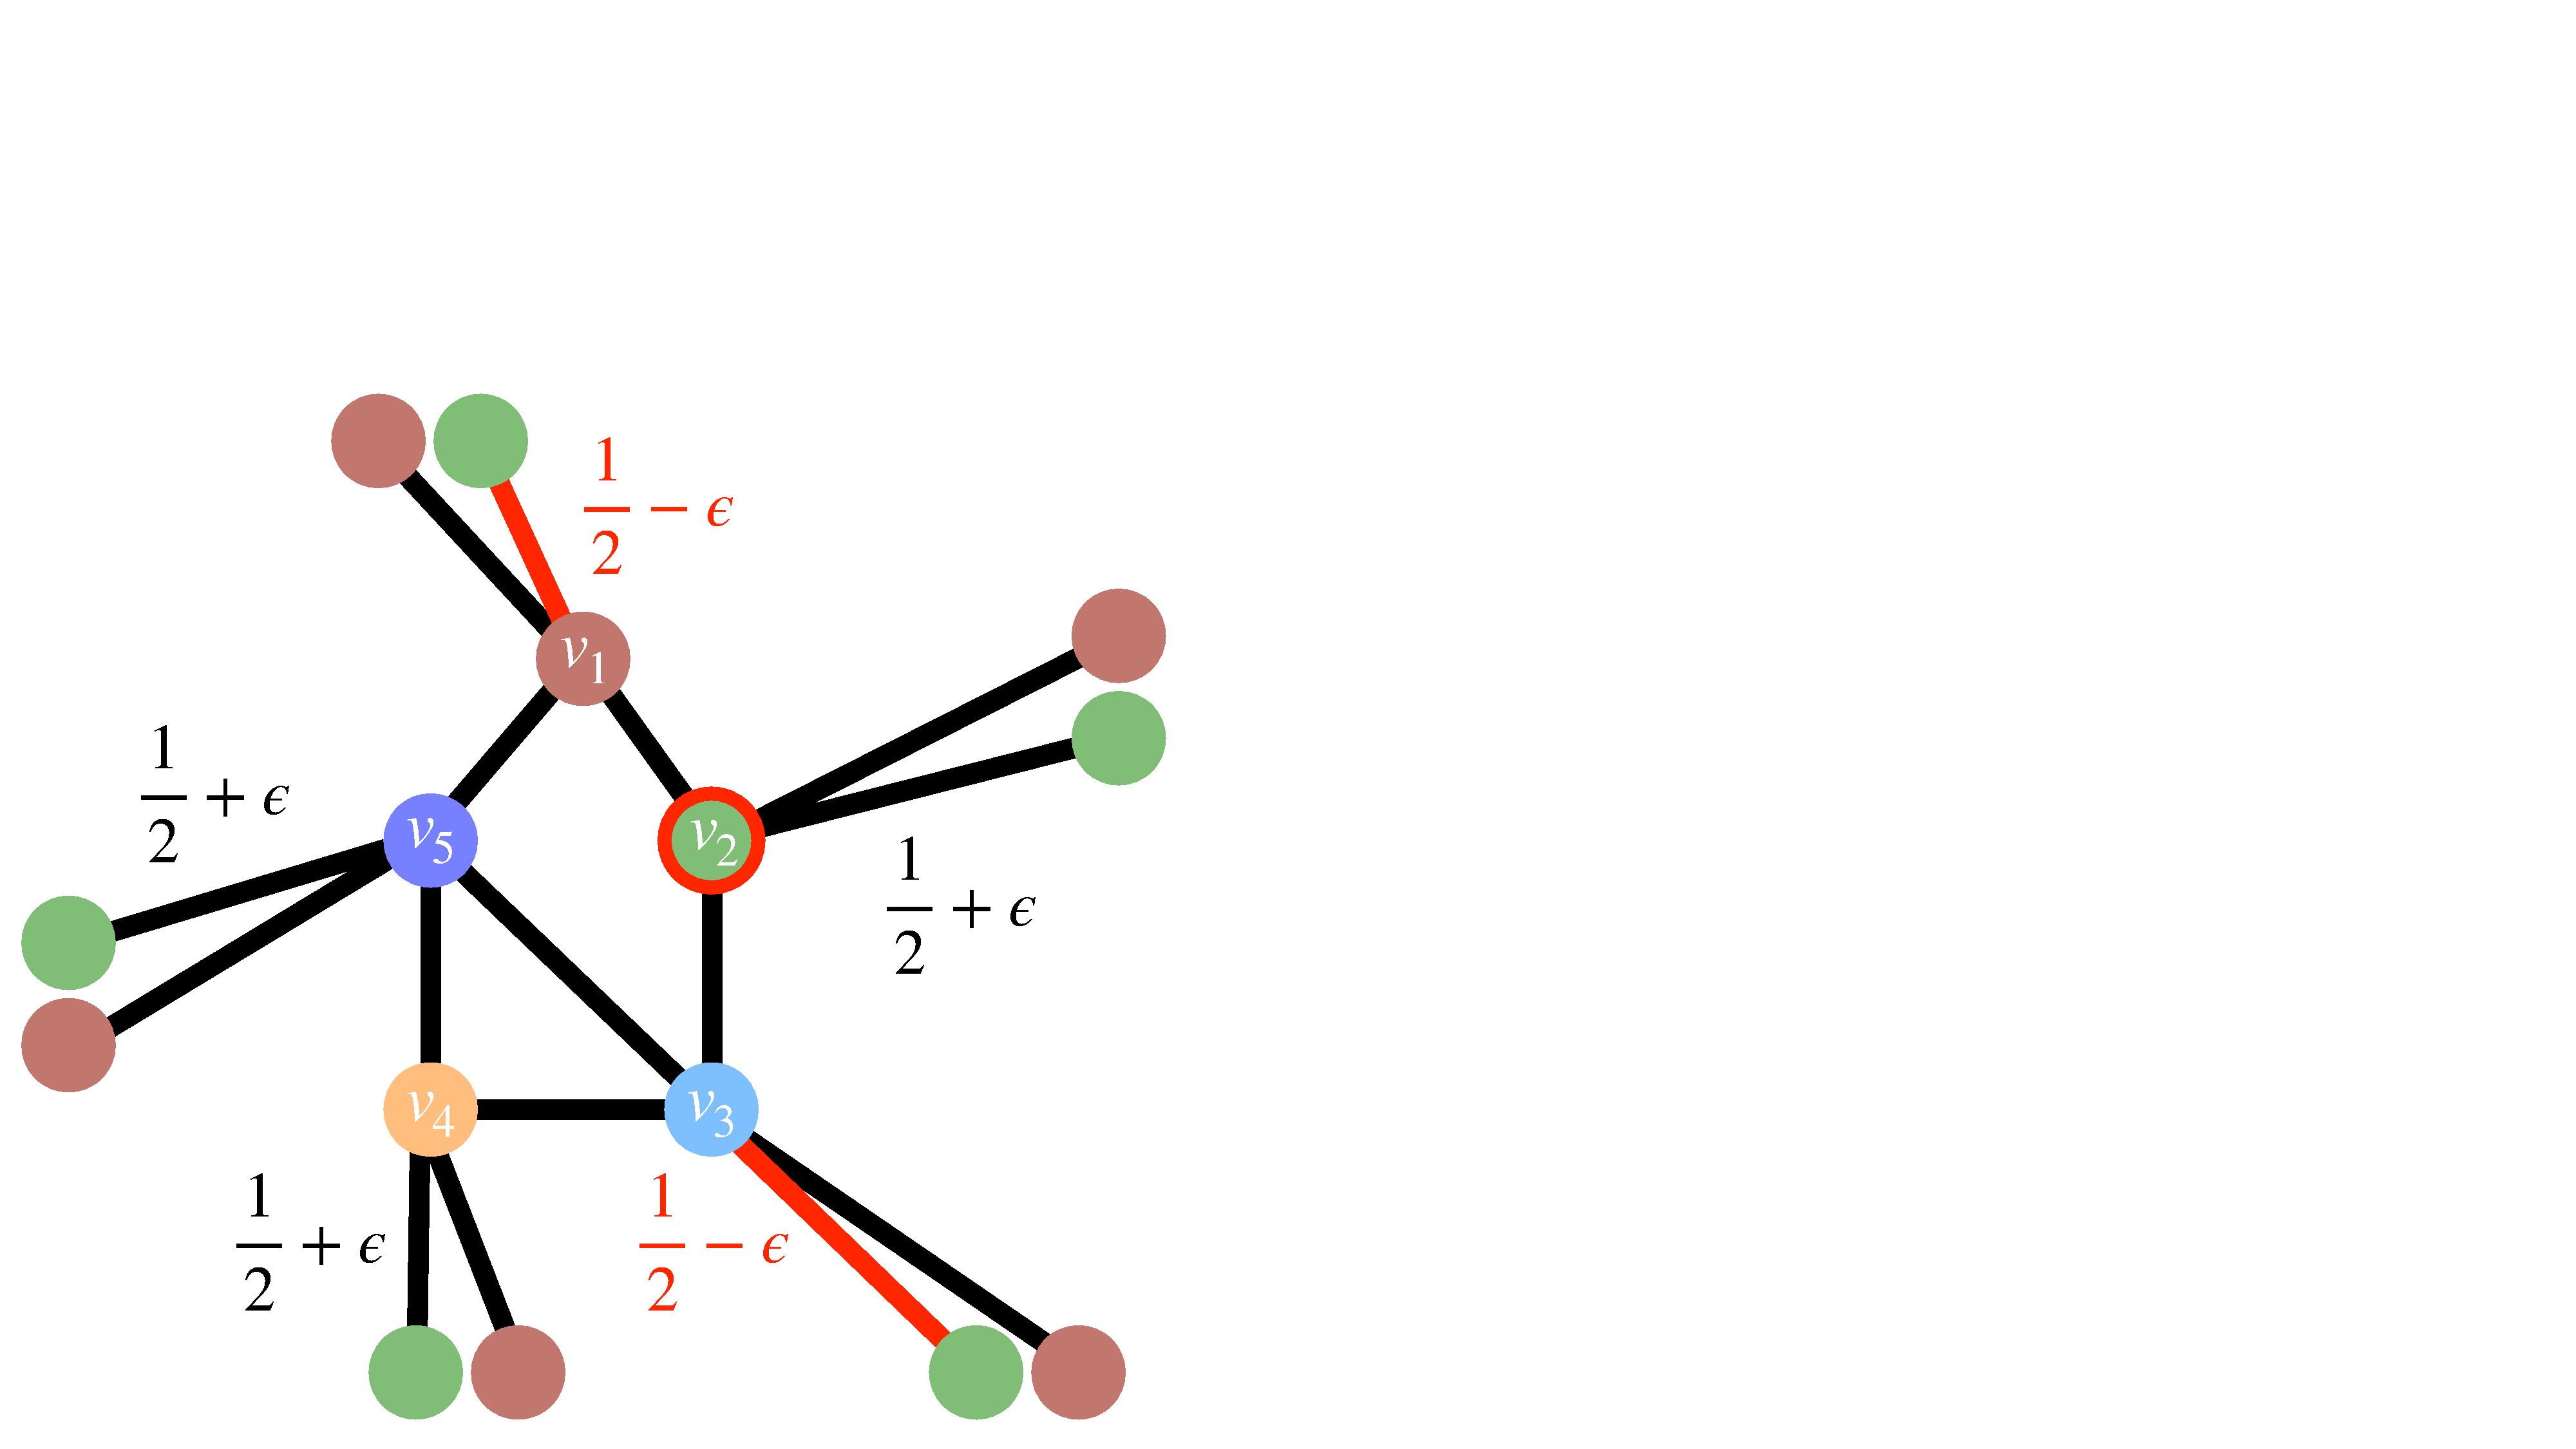
\includegraphics[width=\textwidth,trim=0mm 0mm 370mm 80mm, clip]{./figures/CBMMRed3.pdf}
        \caption{Round $2$.}\label{sfig:CBMMRed3}
    \end{subfigure} \hfill
    \begin{subfigure}[b]{0.25\textwidth}
        \centering
        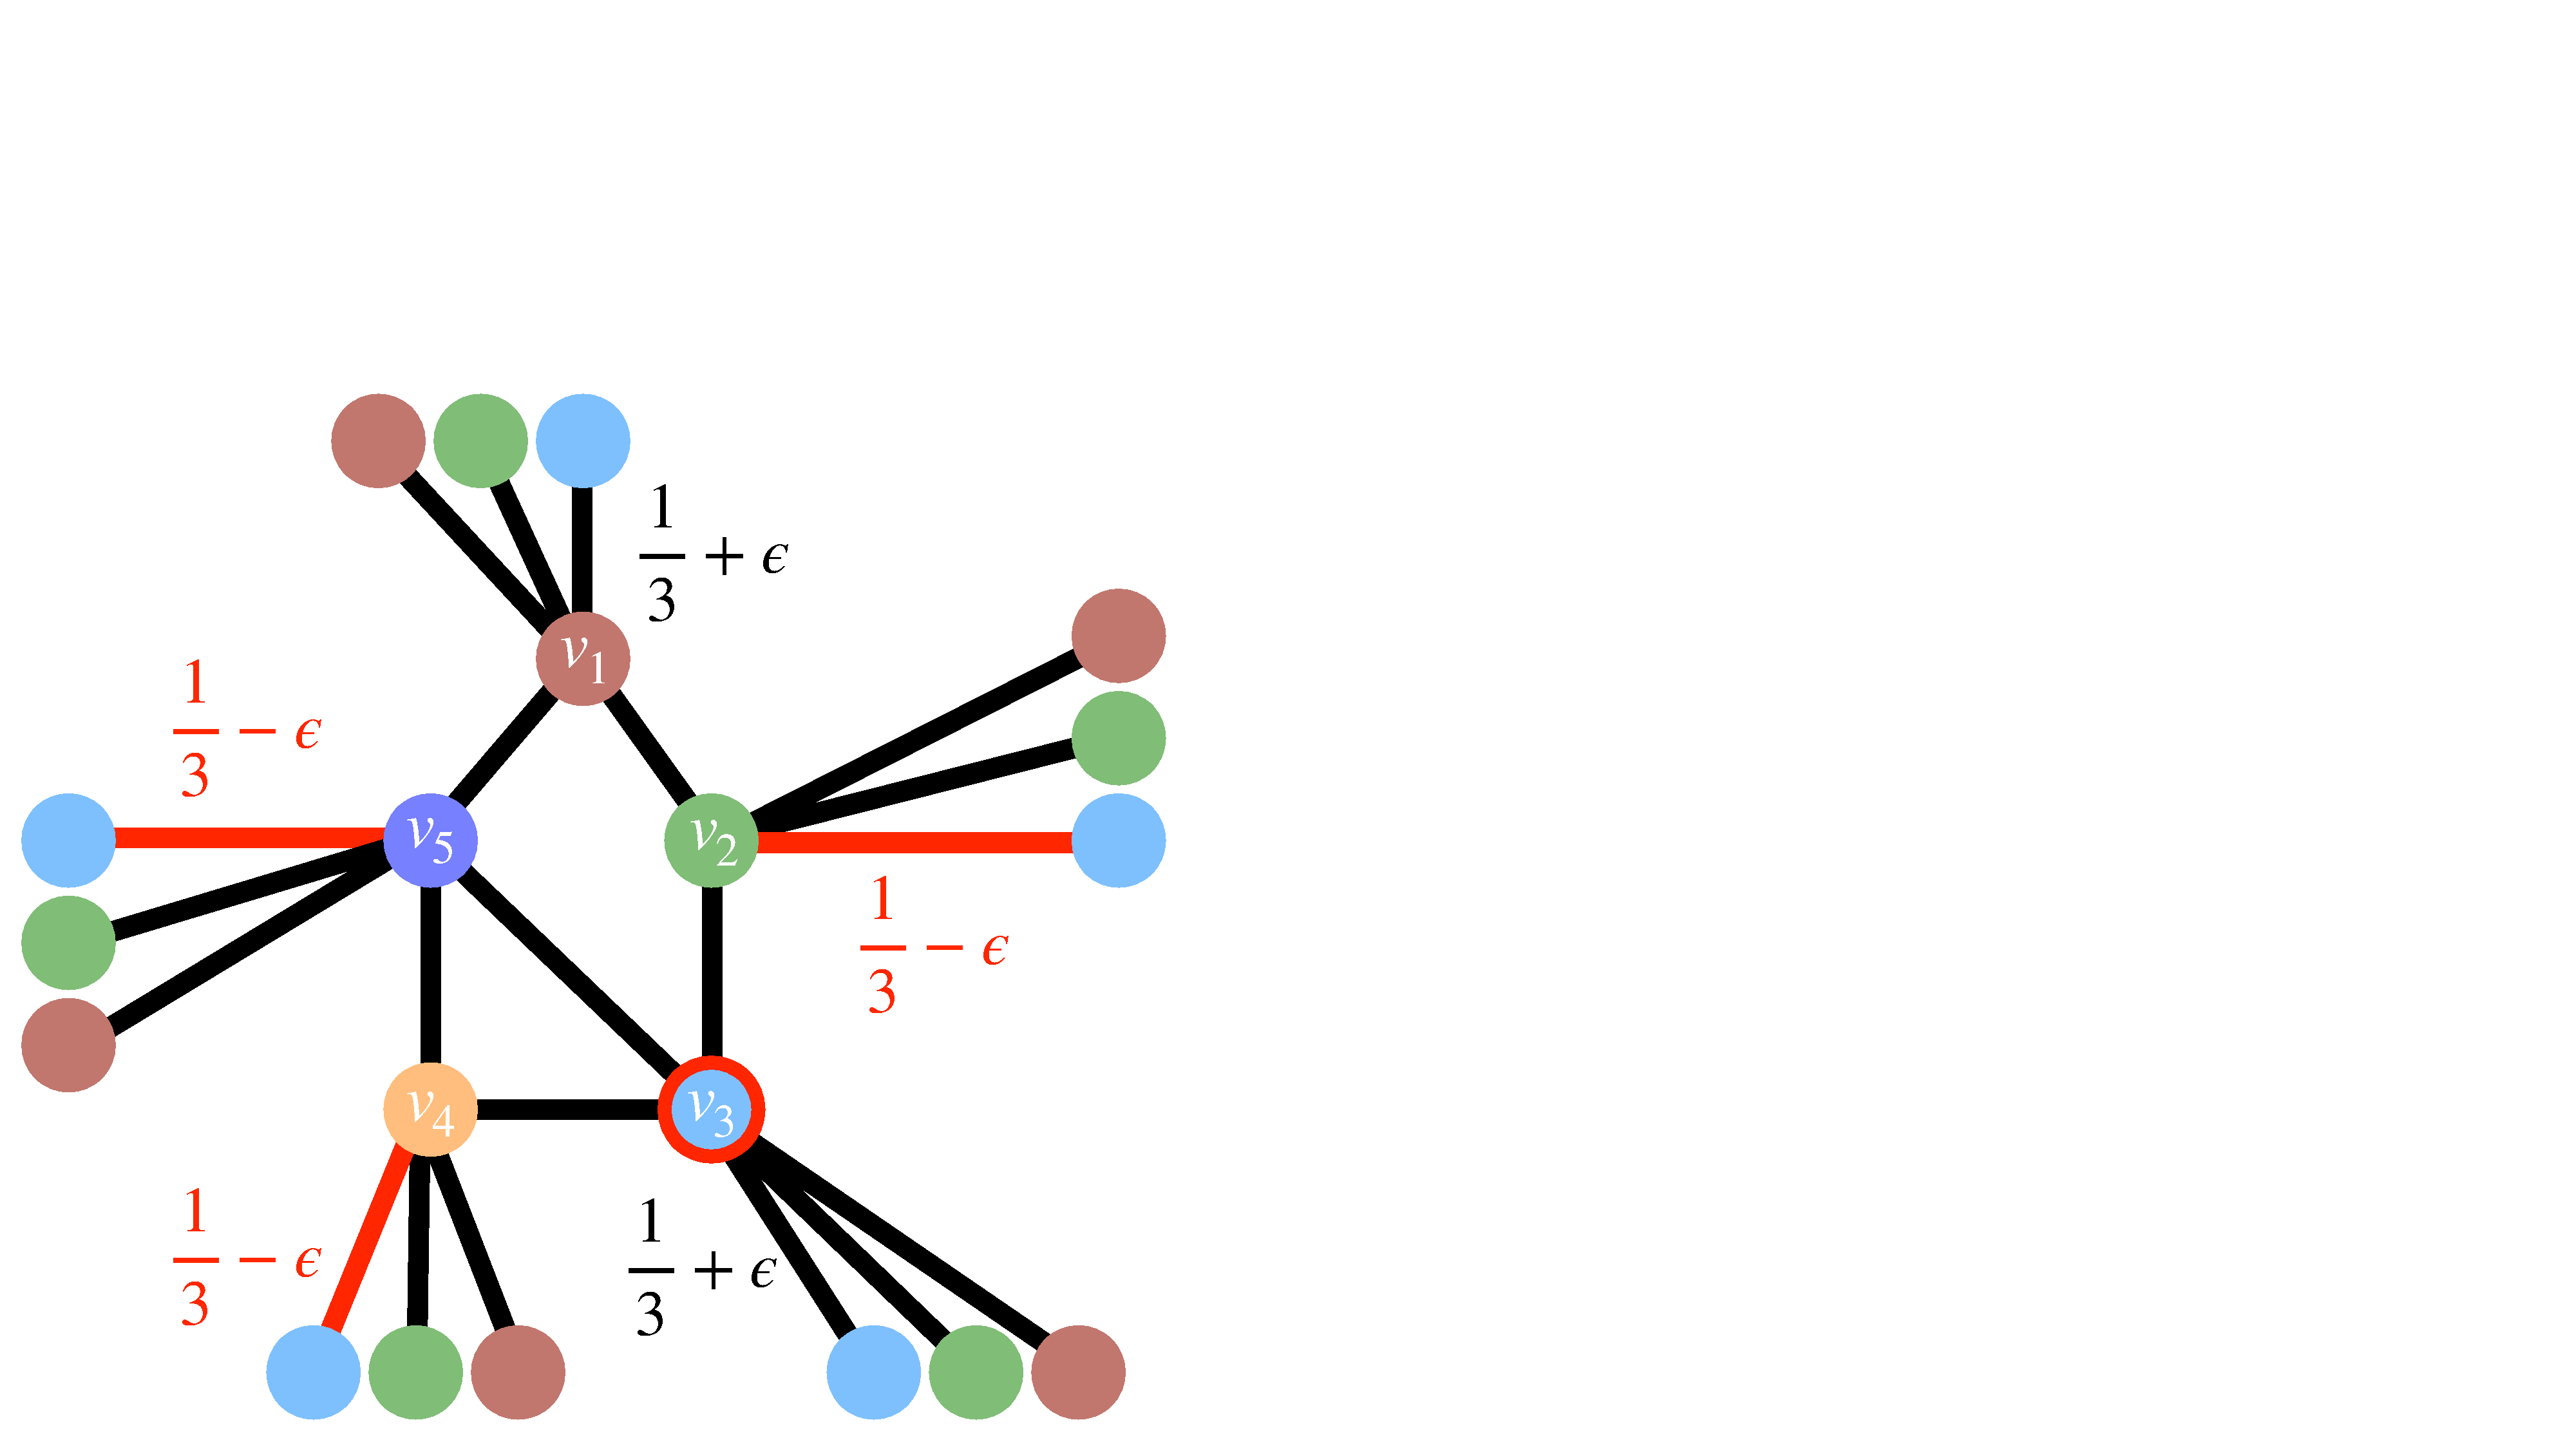
\includegraphics[width=\textwidth,trim=0mm 0mm 370mm 80mm, clip]{./figures/CBMMRed4.pdf}
        \caption{Round $3$.}\label{sfig:CBMMRed4}
    \end{subfigure} \hfill
    \begin{subfigure}[b]{0.25\textwidth}
        \centering
        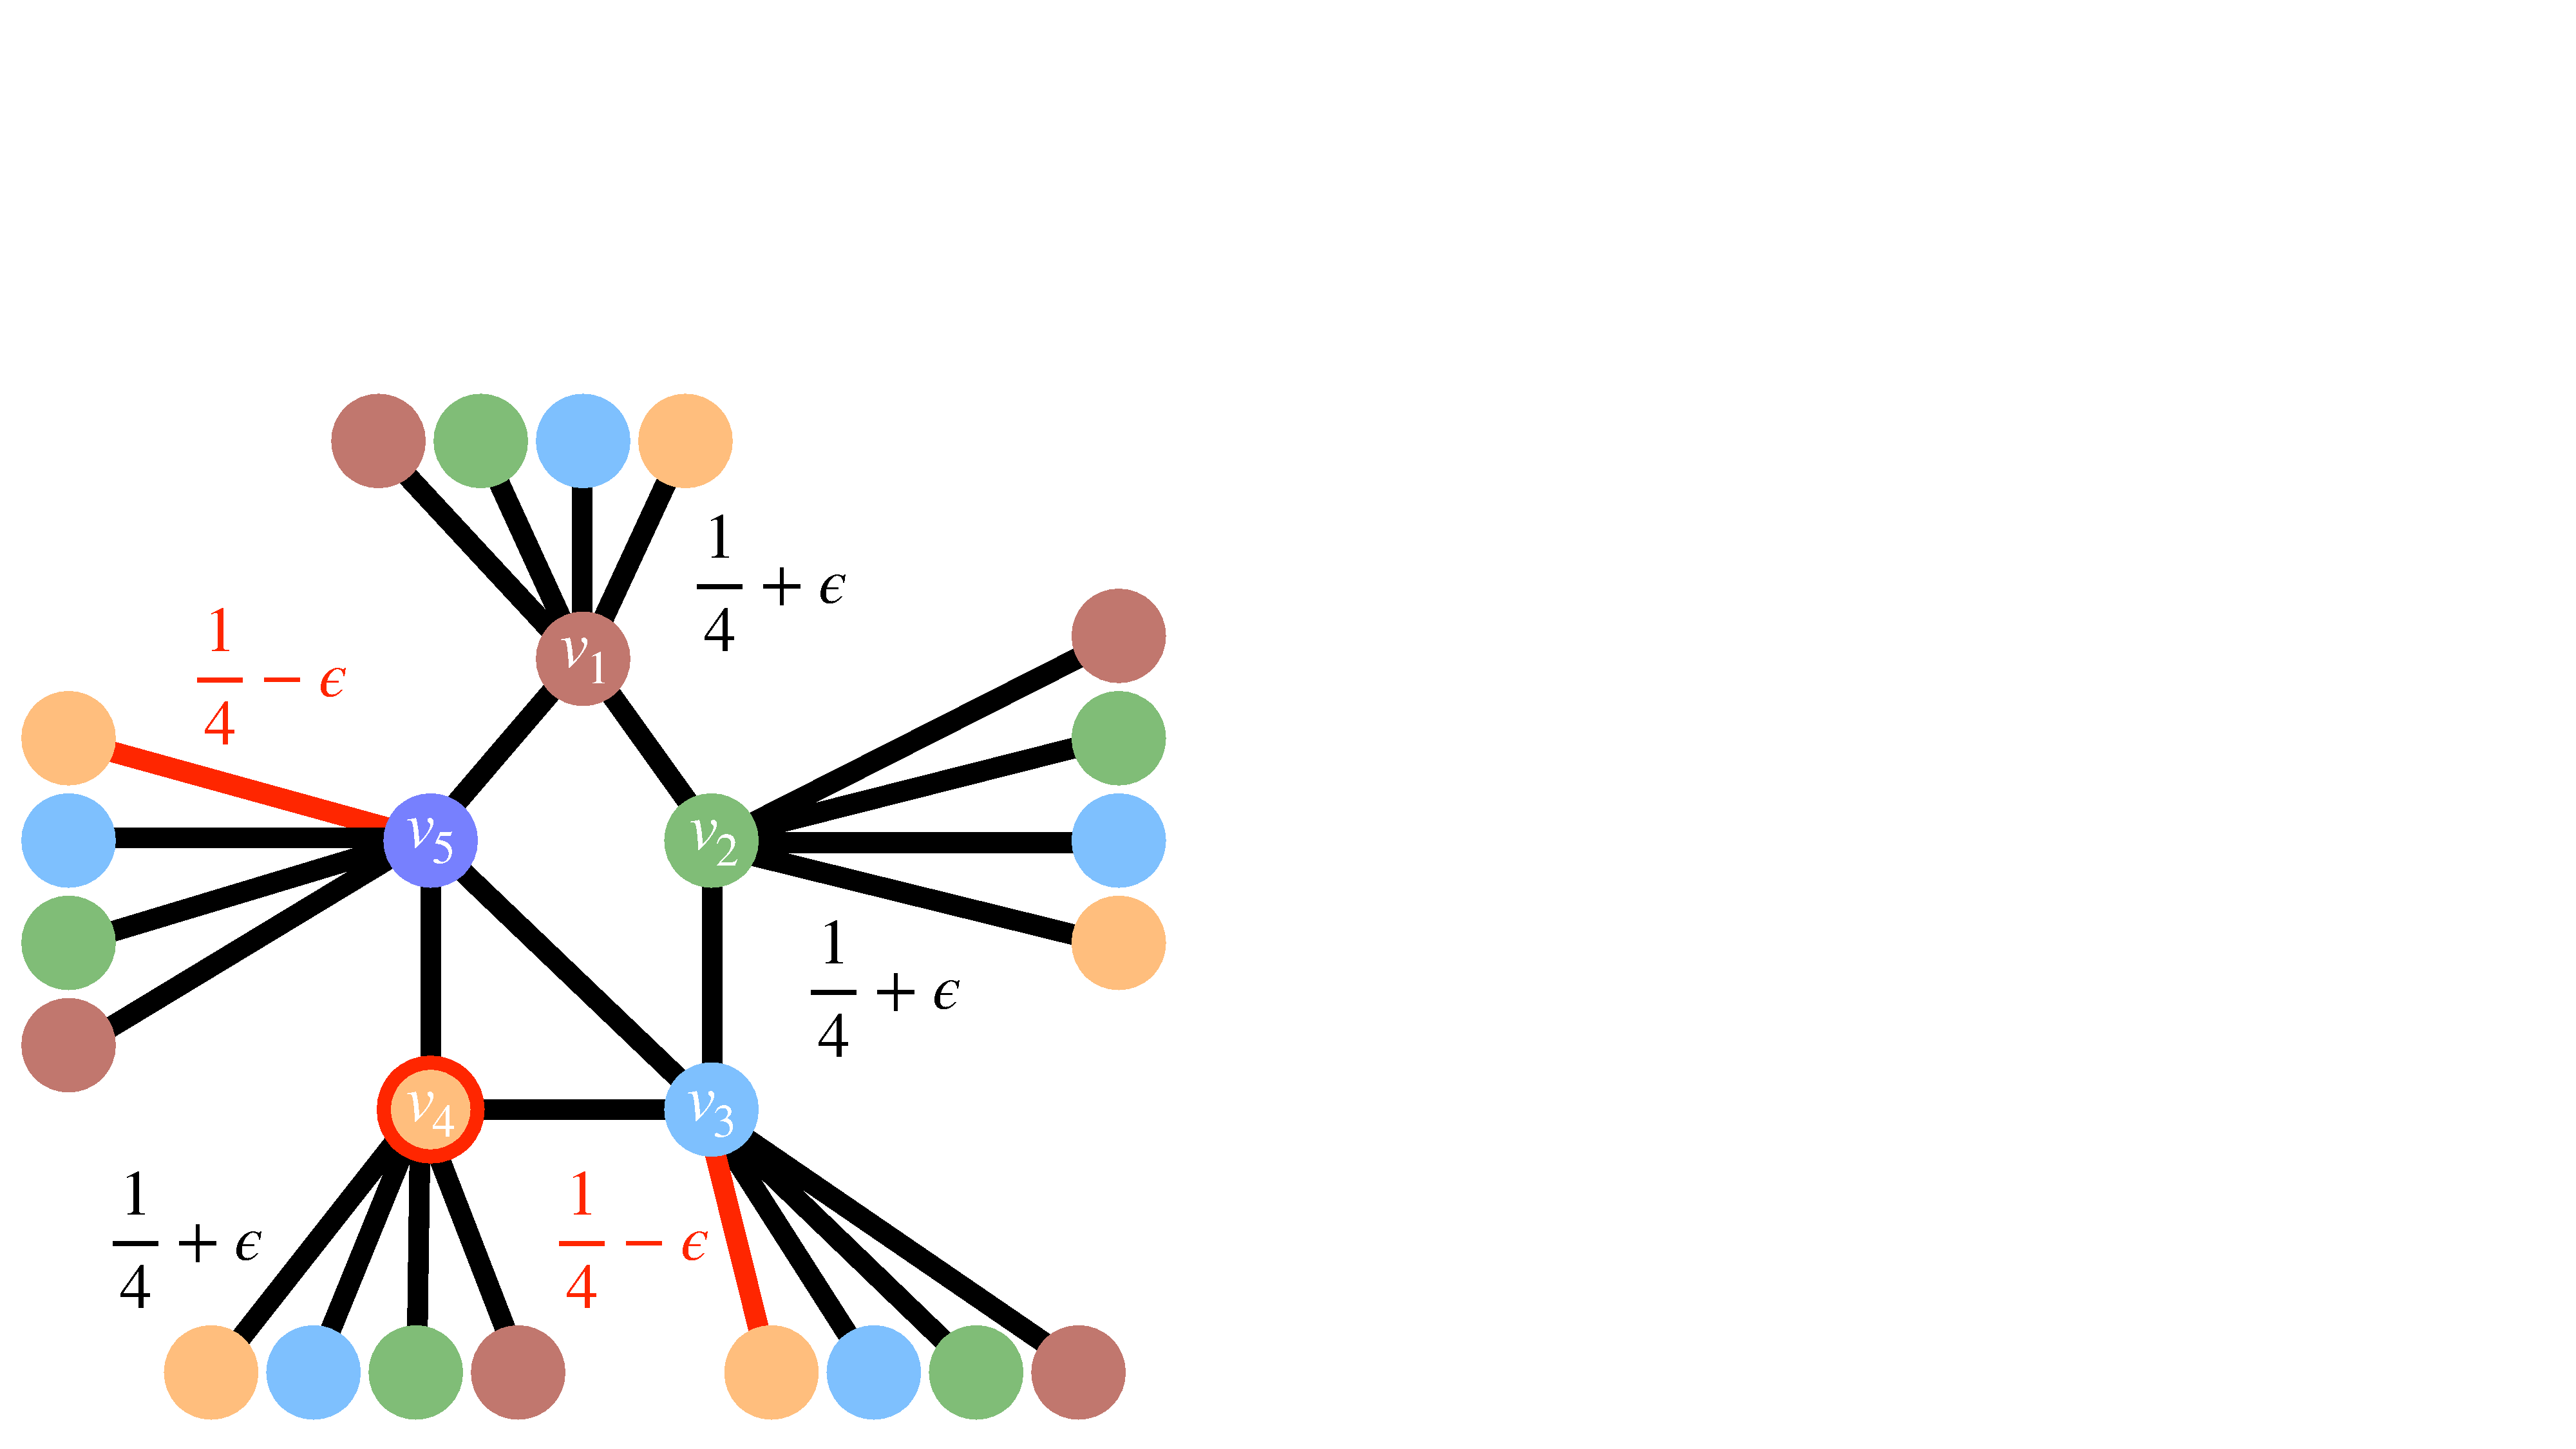
\includegraphics[width=\textwidth,trim=0mm 0mm 370mm 80mm, clip]{./figures/CBMMRed5.pdf}
        \caption{Round $4$.}\label{sfig:CBMMRed5}
    \end{subfigure} \hfill
    \begin{subfigure}[b]{0.25\textwidth}
        \centering
        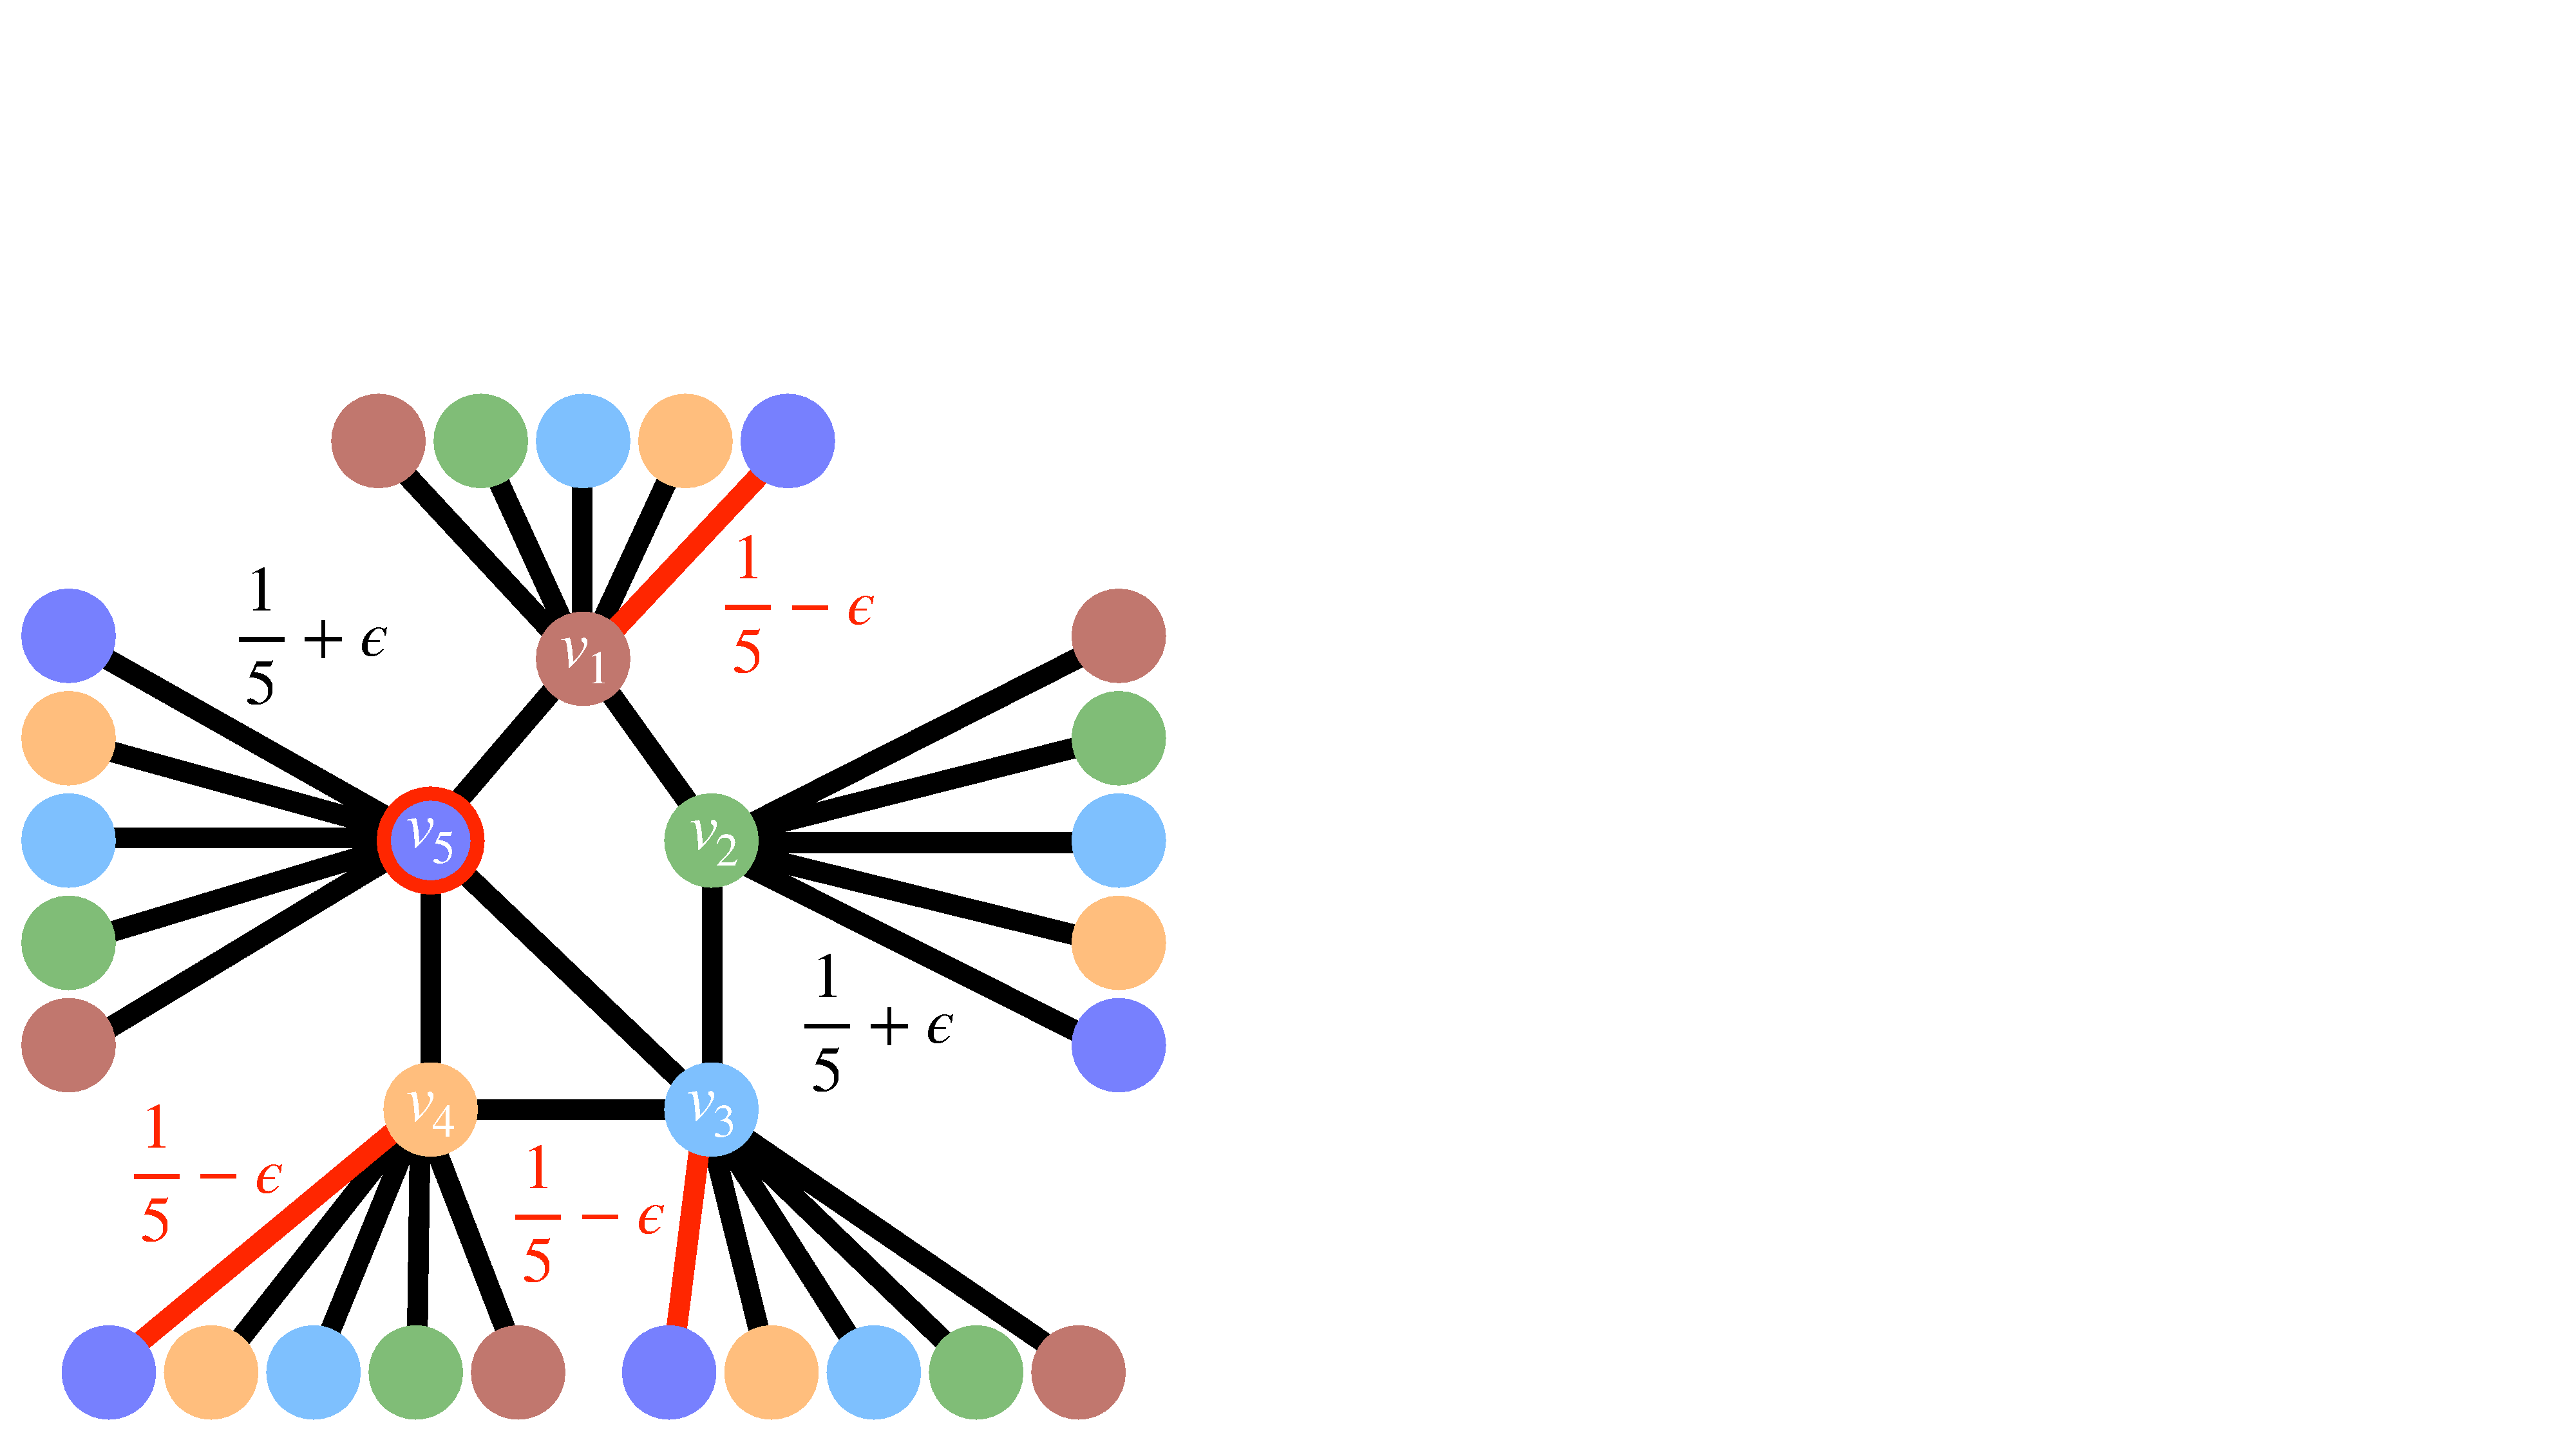
\includegraphics[width=\textwidth,trim=0mm 0mm 370mm 80mm, clip]{./figures/CBMMRed6.pdf}
        \caption{Round $5$.}\label{sfig:CBMMRed6}
    \end{subfigure} \hfill
    \caption{Our triangle detection reduction where we compute $G'$ from $G$ by adding $t=5$ nodes over $t$ rounds. \ref{sfig:CBMMRed6} gives $G'$. Each node labeled according to its round and corresponding vertex in $G$. Edges labelled with their weight in the round they are added (edges of $G$ have weight $1$). For the $i$th round we highlight in red $v_i$ and the edges added with weight $1/i-\epsilon$.} \label{fig:HACSeqRed}
\end{figure}


\paragraph{Running HAC on $G'$}
Having defined $G'$, let us consider the merges that the exact HAC algorithm will make on this instance.
In this section, for succinctness we use {\em weight} to refer to the normalized (i.e., average linkage) weight.
HAC will begin by merging the maximum weight edges.
The maximum weight initially depends on the structure of $N_{G}(v_1)$.
First, all core vertices that are not in $N_{G}(v_1)$ will merge with their round 1 leaves (since these edges have weight $1+\epsilon$) increasing their cluster size to $2$.
This leaves all core vertices in $N_{G}(v_1)$. Any edge in $G'$ between two such core vertices will have weight $1$, and will be merged next.
Crucially, any merge in this round with a weight of $1$ indicates a triangle incident on $v_1$ since the two core vertex endpoints of the edge must be contained in $N_{G}(v_1)$, hence connected by 
edges to $v_1$.
If no edges of weight $1$ merge, the remaining leaves that we added to core vertices in $N_{G}(v_1)$ merge into their neighboring core vertex.

Assuming we did not merge any weight $1$ edges in the first round, at this point the cluster size of each core vertex is $2$, and so the weight of any edge originally in $G$ (between two core vertices) will be $1/4$.
The edge weights to leaves in round $2$ will be $((1/2) \pm \epsilon)/2 = 1/4 \pm (\epsilon / 2)$, which is larger than $1/4$ for edges of Type~\ref{typetwo}.
Therefore, the same argument for how edges merge in round $1$ can be inductively applied to the next round.
The edge weights in round $i$ for edges between core vertices will be $1/i^2$, and by the same argument as before, the Type~\ref{typetwo} (Type~\ref{typeone}) edges will be larger (smaller) by $\epsilon/i$.
%\knote{maybe clarify that the edge weights in round $i$ are $1/i^2$}
As a result of how an exact average linkage HAC will merge the edges of $G'$, we obtain the following lemma:

\begin{lemma}
Consider the sequence of merges performed by the HAC algorithm on $G'$. If the merge sequence consists of $t^2$ merges, which first merge all leaf vertices, and only then makes merges between core vertices, then $G$ does not contain any triangles.
If the merge sequence merges any edge between two core vertices in the first $t^2$ merges, then $G$ contains a triangle.
\end{lemma}

\paragraph{Completing the Reduction}
We will now complete the proof of Theorem~\ref{thm:lbreduction}.
Suppose we are given an instance of \textsc{Triangle Detection} on $n$ vertices.
Conjecture~\ref{conj:bmm} implies that this instance cannot be solved by combinatorial algorithms in $O(n^{3-\epsilon})$ time for any $\epsilon > 0$.

Let the time complexity of HAC on a graph $G$ with $n$ vertices and $m$ edges be $T_{\mathsf{HAC}}(n,m)$.
Suppose HAC can be solved combinatorially in $O(n^{3/2 - \epsilon})$ time.
Given a \textsc{Triangle Detection} instance on $n$ vertices we create a graph $G'$ with $O(n^2)$ vertices and $O(n^2)$ edges, and run HAC on $G'$.
The running time of the reduction is $O(n^2)$, and the running time of HAC on $G'$ is $O((n^{2\cdot (3/2-\epsilon)}) = O(n^{3 - 2\epsilon})$, which will falsify Conjecture~\ref{conj:bmm} by \Cref{thm:bmmeq}.
Thus, conditional on Conjecture~\ref{conj:bmm}, there is no algorithm for HAC running in time $T_{\mathsf{HAC}}(n, m) = O(n^{3/2 - \epsilon})$ for any constant $\epsilon > 0$, completing the proof of Theorems~\ref{thm:lbreduction} and \ref{thm:worklb}. 
The same argument, under the assumption that triangle detection cannot be solved in $O(n^{\omega - \epsilon})$ time for any constant $\epsilon > 0$ implies Theorem~\ref{cor:workmatmul}.




